\section{Magnitude Functions}

In practice, galaxy luminosity is calculated from the \textit{flux} measurement. Flux is measured in $W/m^2$ which is the amount of energy received per second over a given area. However, observing telescopes like the \textit{Spitzer Space Telescope} measure \textit{flux density} through filters that only capture light in specific frequency bands and are measured in \textit{Janksys}. The \gls{zfourge} first measures flux density in $\mu Jy$ which is then converted into \textit{apparent magnitude} using \cref{EQ: Apparent Magnitude}: 

\begin{equation}
    m_{x} = -5 \log_{100} \left(\frac{F_{x}}{F_{x,0}}\right)
    \label{EQ: Apparent Magnitude}
\end{equation}
\myequations{Apparent Magnitude}

where $m_x$ is the apparent magnitude in filter $x$; $F_x$ is the flux density in filter $x$; and $F_{x,0}$ is the reference flux (zero-point) in filter $x$. \gls{zfourge} measures flux density in many bands as mentioned in \cref{Sec: ZFOURGE Overview}. We first test our method of calculating magnitude functions in the $K_{s}$ band. This requires a different method of calculating the \gls{lf} as a few extra steps are required to meet the completeness of the survey. Firstly, the magnitude limit in the $K_{s}$ is $K_{s,lim} = 25.9\ AB$. Apparent magnitudes can be converted to \textit{AB magnitudes} with \cref{EQ: AB Magnitude}:

\begin{equation}
    M_{AB} = 25 - 2.5 \log_{10}(m)
    \label{EQ: AB Magnitude}
\end{equation}
\myequations{AB Magnitude}

Finally, AB magnitude is converted into \textit{absolute magnitude} which is the apparent magnitude a celestial object would have if it were located at a distance of 10 parsecs and is given by \cref{EQ: Absolute Magnitude}:

\begin{equation}
    M_{abs} = M_{AB} - 5 \log_{10} \left(\frac{d}{10}\right)
    \label{EQ: Absolute Magnitude}
\end{equation}
\myequations{Absolute Magnitude}

Where $d$ is distance measured in units of parsecs. We calculate the distance to each galaxy using the \texttt{Astropy} python package \citep{astropy_collaboration_astropy_2022}. Speciically, the following python code is used:

\vspace{12pt}
\begin{python}    
    # Cosmology
    cosmo = FlatLambdaCDM(H0=70, Om0=0.3)
    
    # Luminosity distance
    d_c = cosmo.comoving_distance(z) * 10 ** 6 # Mpc -> pc
\end{python}

Where $z$ is the photometric redshift, or spectroscopic redshift if available, of each galaxy. The \texttt{luminosity\_distance} $(d_L)$ and \texttt{comoving\_distance} $(d_C)$ measure two separate distances. $d_C$ does not factor the expansion of the universe and is especially useful in \gls{lf} calculations because it keeps the volume of observed space consistent (\cref{EQ: Vmax}) across all cosmic time. Otherwise, $d_L$ will include the expansion of the universe which inherently disperses galaxies and leads to incorrect number density calculations (\cref{EQ: Number Density}). However, $d_L$ is still useful because it can be used as a completeness limit. \Cref{Fig: Magnitude Distribution} shows the absolute magnitude calculated with both $d_C$ and $d_L$. The apparent magnitude limit in the $K_{s}$ band is applied and masks galaxies with AB magnitudes fainter than $25.9$ because the units are the same, creating the hard edge. Galaxies with absolute magnitudes fainter (more positive; above) than the hard edge created by $d_L$ do not meet the completeness limit. 

\begin{figure}[t!]
    \centering
    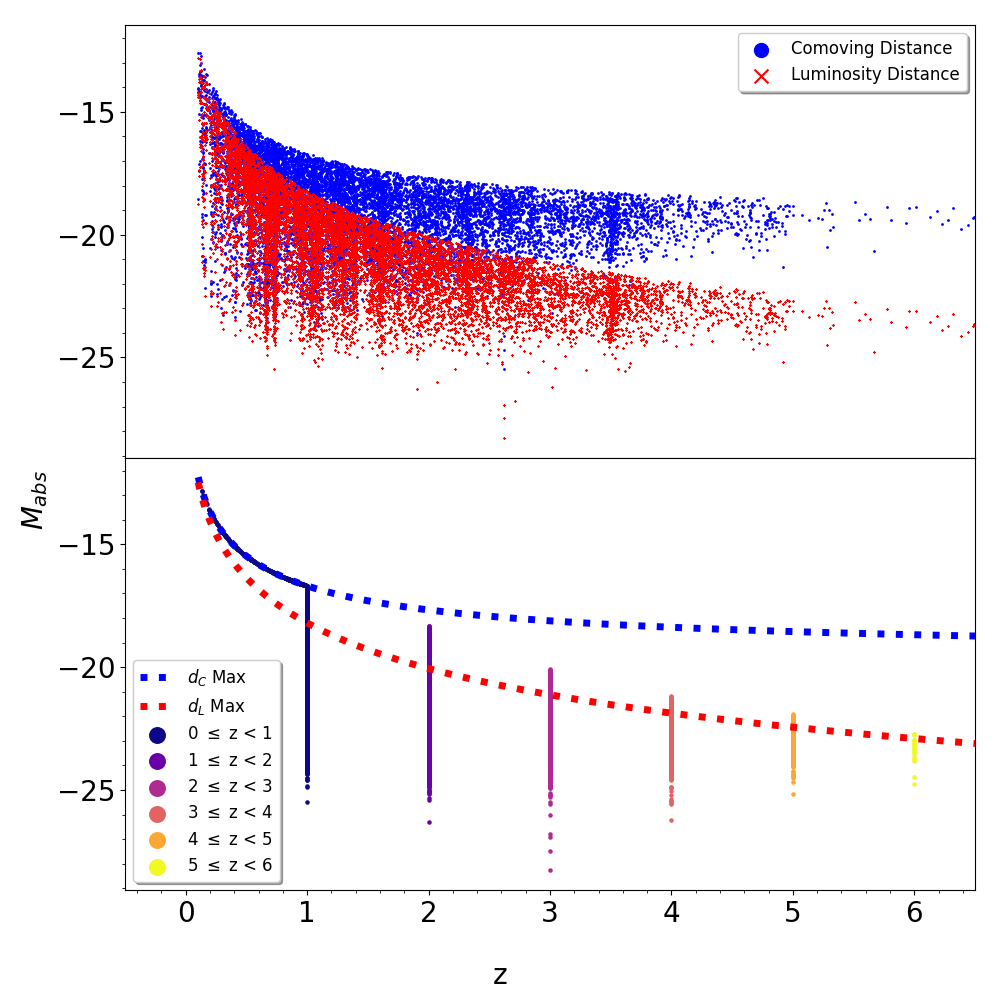
\includegraphics[width=\textwidth]{Figures/Magnitude Distribution.png}
    \caption{ZFOURGE CDFS $K_s$ band magnitude distribution as a function of redshift. Galaxies are masked with $K_{s,lim}$. \textit{Top:} magnitudes calculated with $d_C$ and $d_L$. \textit{Bottom:} the maximum distance of each galaxy according to the redshift bin it resides in.}
    \label{Fig: Magnitude Distribution}
\end{figure}

$D_{max}$ refers to the distance an object would appear at given it has the same magnitude but if the flux density was at the detectable threshold of the survey. Decreasing flux, but keeping luminosity constant, means that distance must be the variable changing (increasing). Rearranging \cref{EQ: Absolute Magnitude}, distance can be swapped for $d_{max}$ if $M_{AB}$ is replaced with the magnitude limit. In this case the magnitude limit is $K_{s,lim} = 25.9$ and $d_{max}$ is given by \cref{EQ: Magnitude Dmax}:

\begin{equation}
    d_{max}\ [pc] = 10 \times 10^{\textstyle{\left(\frac{K_{s,lim} - M_{abs}}{5}\right)}}
    \label{EQ: Magnitude Dmax}
\end{equation}
\myequations{Magnitude $d_{max}$}

The maximum comoving distance of each galaxy is then calculated. \Cref{Fig: Magnitude Distribution} (bottom) displays the maximum $d_C$ distance. Galaxies above the $d_L$ maximum line are outside the completeness limit and are removed. Only the first redshift bin, $0 \leq z < 1$, has galaxies faint enough such that their maximum distance does not reach the end of the redshift bin. After removing sources outside the completeness limit, the maximum comoving distance of each galaxy is the end of the redshift bin it resides in. 

\begin{figure}[b!]
    \centering
    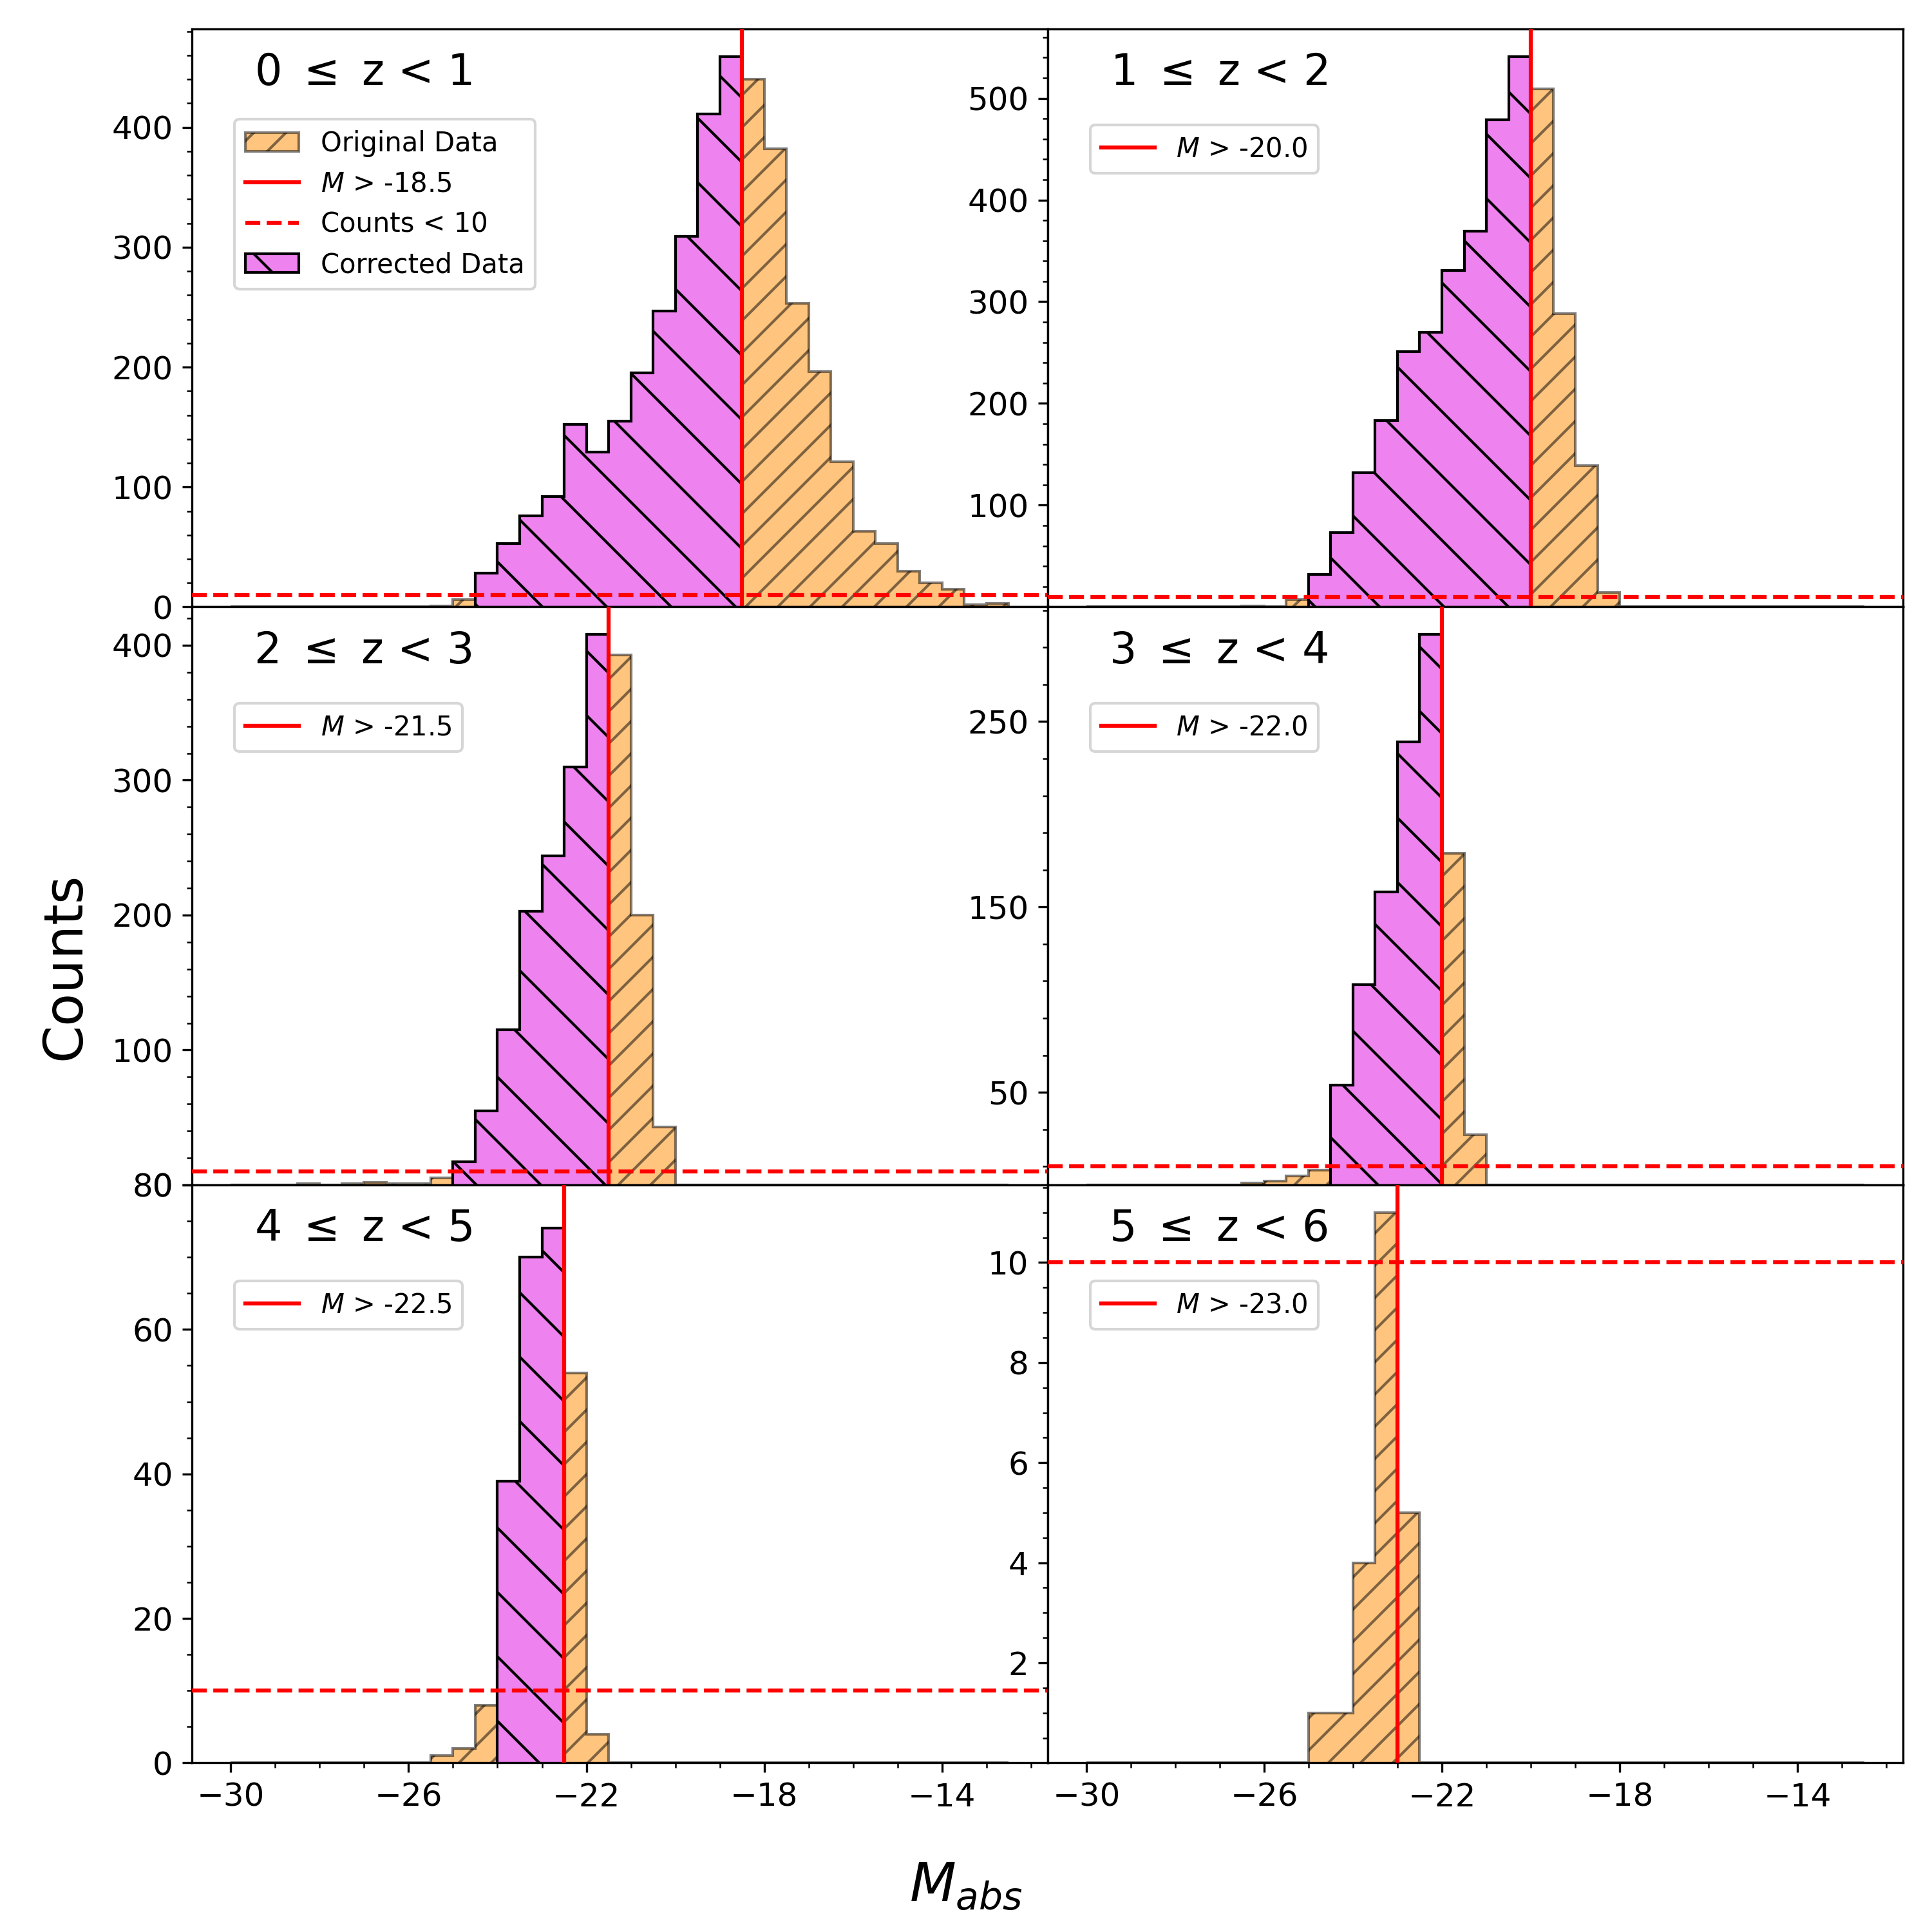
\includegraphics[width=\textwidth]{Figures/Magnitude Counts.png}
    \caption{Number counts in each redshift and luminosity bin. The blue dashed vertical line represents the completeness limit. The red dashed horizonal line shows that each luminosity bin requires at least 10 galaxies or it is discarded. Purple bins show the corrected data.}
    \label{Fig: Magnitude Counts}
\end{figure}

Using $d_L$ as the completion limit works extremely well. Otherwise, there is a turn-over in the number counts as seen in \cref{Fig: Magnitude Counts}. This corrected number counts figure represents the shape that the \gls{lf} will take. Bins coloured orange are below the completeness limit and as such are too faint. Purple bins are complete and will be used to calculate the \gls{lf}. The completeness limit is represented by the blue dashed vertical line. Bins are also discarded if the number of galaxies is less than 10. The final redshift bin, $5 \leq z < 6$, is entirely masked as no bin has more than 10 sources. The decision to use equally spaced reshift bins was to simplify the testing process. A number of various redshift bin sizes are chosen in the literature, such as equal spacing in \textit{look-back time} \citep{thorne_deep_2022}. 